\documentclass[floatfix,nofootinbib,superscriptaddress,fleqn]{revtex4-2}  
%\documentclass[aps,epsfig,tightlines,fleqn]{revtex4}
\usepackage[utf]{kotex}
\usepackage[HWP]{dhucs-interword}
\usepackage[dvips]{color}
\usepackage{graphicx}
\usepackage{bm}
%\usepackage{fancyhdr}
%\usepackage{dcolumn}
\usepackage{defcolor}
\usepackage{amsmath}
\usepackage{amsfonts}
\usepackage{amssymb}
\usepackage{amscd}
\usepackage{amsthm}
\usepackage[utf8]{inputenc}
 \usepackage{setspace}
 \usepackage{tikz}
 \usepackage{pgf}
 
%\pagestyle{fancy}

\begin{document}

\title{\Large 2022년 1학기 물리학 I: Quiz 15}
\author{김현철\footnote{Office: 5S-436D (면담시간 매주
    화요일-16:00$\sim$20:00)}} 
\email{hchkim@inha.ac.kr}
\author{Lee Hui-Jae} 
\email{hjlee6674@inha.edu}
\affiliation{Hadron Theory Group, Department of Physics,
Inha University, Incheon 22212, Republic of Koreaw }
\date{Spring semester, 2022}


\vspace{1.cm}

\maketitle


\noindent {\bf 문제 1. (30 pt)} 
그림~\ref{fig:1}처럼 질량 $m=0.85$ kg, 반지름 $r=4.2$ cm인 균일한 공이,
쓸림이 없는 벽에 고정되어있고 질량이 없는 줄에 매달려 있다. 공의
질량중심과 줄 끝 사이의 수직거리가 $L=8.0$ cm일 때
\begin{figure}[htp]
  \centering
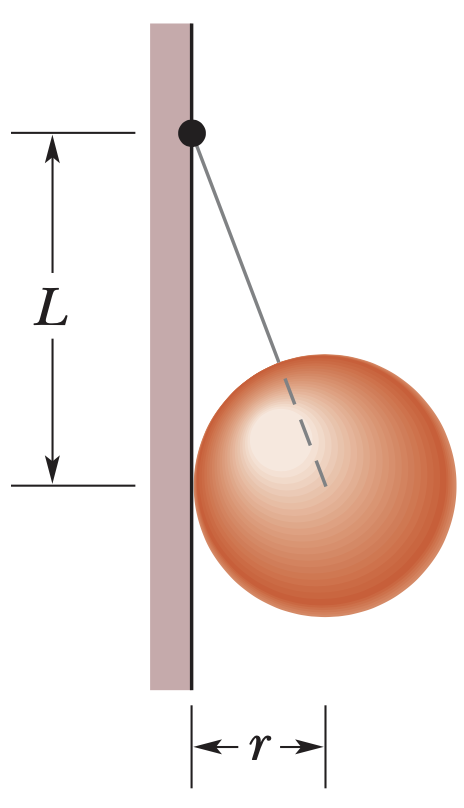
\includegraphics[scale=0.5]{Qfig15-1-20220502.png}
  \caption{문제 1}
  \label{fig:1}
\end{figure}
\begin{itemize}
\item[(가)] 줄에 걸리는 장력과
\item[(나)] 벽이 공에 가하는 힘을 각각 구하여라. 
\end{itemize}

\noindent {\bf 풀이 : } 
공에 작용하는 수직항력을 $N$, 장력을 $T$라 하자. 중력은 $mg$만큼 
작용하므로 공의 자유 물체 다이어그램을 그려보면 다음과 같다.
\begin{figure}[htbp]
  \centering
  \begin{tikzpicture}
    \draw (0,-2) -- (0,2); 
    \draw (-2.5,0) -- (2.5,0);
    \draw [blue,very thick,-latex] (0.1,0)--(1.5,0) 
            node [above=2,black] {$N$};

    \draw[red,very thick,-latex] (0,-0.1) -- (0,-1.8) 
    node [left,black] {$mg$};

    \draw[rotate=30,blue,very thick,-latex] (0,0.1)--(0,1.2)
    node [above,black] {$T$};
  \end{tikzpicture}
\end{figure} 

줄과 벽이 이루는 각도를 $\theta$라 하면
운동 방정식을 다음과 같이 기술할 수 있다.
\begin{align}
  \label{eq:1-1}\sum F_x &= N-T\sin\theta =0, \\
  \label{eq:1-1-1}\sum F_y &= T\cos\theta -mg =0.
\end{align}

\begin{itemize}
  \item[(가)] 식 \eqref{eq:1-1}과 \eqref{eq:1-1-1}에 의해 $T$는
  \begin{align}
    T = \frac{mg}{\cos\theta}
  \end{align}
  이고 $\theta$는 줄과 벽 사이 각도이므로
  \begin{align}
    \cos\theta = \frac{L}{\sqrt{L^2+r^2}}
  \end{align}
  이다. 따라서 장력 $T$는 다음과 같이 계산하여 얻을 수 있다.
  \begin{align}
    \begin{split}
      T &=\frac{mg\sqrt{L^2+r^2}}{L}
      = \frac{(0.85\,\mathrm{kg})(9.80\,\mathrm{m/s^2})
      \sqrt{((8.0\times 10^{-2}\,\mathrm{m})^2
      +(4.2\times 10^{-2}\,\mathrm{m})^2}}
      {(8.0\times 10^{-2}\,\mathrm{m})} \\
      &= 9.4\,\mathrm{N}.
    \end{split}
  \end{align}
  장력의 크기는 $9.4\,\mathrm{N}$이다.
  \item[(나)]
  식 \eqref{eq:1-1-1}로부터 벽에 의한 수직항력 $N$은
  \begin{align}
    N =T\sin\theta =\frac{mg}{\cos\theta}\sin\theta=mg\tan\theta
    =mg\frac{r}{L} 
  \end{align}
  이다. 따라서 수직항력은 다음과 같이 계산하여 얻을 수 있다.
  \begin{align}
    \begin{split}
      N &=mg\frac{r}{L} 
      = (0.85\,\mathrm{kg})(9.80\,\mathrm{m/s^2})
      \frac{(4.2\times 10^{-2}\,\mathrm{m})}
      {(8.0\times 10^{-2}\,\mathrm{m})} \\
      &= 4.4\,\mathrm{N}.
    \end{split}
  \end{align}
  수직항력의 크기는 $4.4\,\mathrm{N}$이다.
\end{itemize}

\vspace{0.5cm}

\noindent {\bf 문제 2. (30 pt)}
그림~\ref{fig:2}에서 바위를 타는 질량 55 kg인 사람이 손으로 바위틈 한
쪽을 잡아당기고 발로는 바위틈 반대쪽을 누르면서 ``뒤로 기대 오르기''를
하고 있다. 바위틈은 폭이 $w=0.20$ m이고, 사람의 질량 중심은 바위틈에서
수평으로 $d=0.40$ m의 거리에 있다. 정지마찰계수는 손과 바위 사이가
$\mu_1=0.40$이고 신발과 바위 사이는 $\mu_2=1.2$이다.  
\begin{figure}[ht]
  \centering
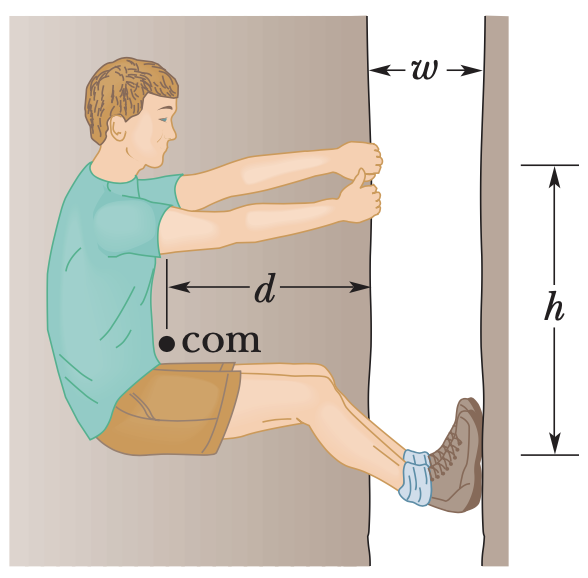
\includegraphics[scale=0.6]{Qfig15-2-20220502.png}
  \caption{문제 2}
  \label{fig:2}
\end{figure}
\begin{itemize}
\item[(가)] 사람이 안정되게 있기 위해서 손과 발이 각각 수평하게 가해야
  하는 최소한의 힘은 얼마인가?
\item[(나)] (가)와 같은 힘의 경우 손과 발 사이의 수직거리 $h$는
  얼마인가?
\item[(다)]  바위가 젖어서 $\mu_1$, $\mu_2$가 작아지면, (가)의
  답과
\item[(라)] (나)의 답은 어떻게 달라질까?
\end{itemize}

\noindent {\bf 풀이 : } 손에 작용하는 수직항력과 정지마찰력을 각각 
$N_1$, $f_{s1}$,
발에 작용하는 수직항력과 정지마찰력을 $N_2$, $f_{s2}$라 하고 
사람에게 작용하는 중력을 
$F_g$라 하자. 작용점을 고려하여 사람에게 작용하는 힘을 
다음과 같이 성분별로 나누어 그릴 수 있다.

\begin{figure}[htbp]
  \centering
  \begin{tikzpicture}
    \draw (-2,2) node [] {$x$ 축 방향 : };
    \draw[blue,very thick,-latex] (0,-2)--(-2.4,-2)
    node [left,black] {$N_2$};
    \draw[blue,very thick,-latex] (0,1.6)--(1.6,1.6)
    node [right,black] {$N_1$};
    \draw[fill] (0,-2) circle (2pt) node [right,black] {$A$};
    \draw[thick] [|<->|] (0,-2)--(0,1.6) node [midway,left] {$h$};
  \end{tikzpicture}
  \centering
  \begin{tikzpicture}
    \draw (-2,2) node [] {$y$ 축 방향 : };
    \draw[fill] (-1.6,0) circle (2pt) node [above,black] {com};
    \draw[red,very thick,-latex] (-1.6,0) -- (-1.6,-2) 
    node [left,black] {$F_g$};
    \draw[red,very thick,-latex] (0.5,0)--(0.5,1.6)
    node [left,black] {$f_{s1}$};
    \draw[fill] (1.6,0) circle (2pt) node [below,black] {$A$};
    \draw[red,very thick,-latex] (1.6,0)--(1.6,1.6)
    node [right,black] {$f_{s2}$};
    \draw[thick] [|<->|] (-1.6,0)--(0.5,0) node [midway,below] {$d$};
    \draw[thick] [<->|] (0.5,0)--(1.6,0) node [midway,below] {$w$};
  \end{tikzpicture}
  \caption{각 방향으로 작용하는 힘}
\end{figure} 

점 $A$는 발과 벽이 닿는 지점이다.
운동 방정식을 적어보면 다음과 같다.
\begin{align}
  \label{eq:2-1}\sum F_x &= N_{2}-N_{1} = 0,  \\
  \label{eq:2-1-1}\sum F_y &= f_{s1}+f_{s2}-F_g = 0.
\end{align}
사람은 정지해있기 위해 각 방향의 합력은 $0$이어야 한다.
\begin{itemize}
  \item[(가)] 마찰력은 수직항력에 비례하므로
  \begin{align}\label{eq:2-1-2}
    f_{s1} = \mu_1N_1,\,\,\,
    f_{s2} = \mu_2N_2.
  \end{align}
  이다. 식~\eqref{eq:2-1},~\eqref{eq:2-1-2}에 의해 
  식~\eqref{eq:2-1-1}은
  \begin{align}
    (\mu_1+\mu_2)N_1 =F_g
  \end{align}
  으로 고쳐 쓸 수 있다.
  $N_1$은 중력보다 커야하므로 최소한의 $N_1$은 중력과 같아야 한다. 즉,
  \begin{align}\label{eq:2-2}
    \begin{split}
      N_1 &= \frac{mg}{\mu_1+\mu_2}
      = \frac{(55\,\mathrm{kg})(9.8\,\mathrm{m/s^2})}{0.40+1.2} \\
      &= 3.4\times\,10^2\,\mathrm{N}
    \end{split}
  \end{align}
  이다. 손과 발이 수평하게 가해야 하는 최소한의 힘은 
  $3.4\times\,10^2\,\mathrm{N}$이다.
  \item[(나)] 
  사람은 정지해있기 위해서는 돌림힘의 합이 $0$이어야 한다. 
  발과 벽이 닿아 있는 점 $A$를 회전축으로 하여
  돌림힘 계산해보자.
  \begin{align}
    \sum \tau = N_1 h + f_{s1} w - F_g(w+d) = 0
  \end{align}
  $h$에 대해 정리하면
  \begin{align}\label{eq:2-3}
    h = \frac{F_g(w+d)-f_{s1} w}{N_1}
    =\frac{mg(w+d)-\mu_1N_1 w}{N_1}
    =(w+d)(\mu_1+\mu_2) - \mu_1 w
  \end{align}
  이다. 수치를 넣어 값을 계산하자.
  \begin{align}
    \begin{split}
      h=((0.20\,\mathrm{m})+(0.40\,\mathrm{m}))(0.40+1.2) 
      - (0.40)(0.20\,\mathrm{m})
      =0.88\,\mathrm{m}.
    \end{split}
  \end{align}
  손과 발 사이 수직거리는 $0.88\,\mathrm{m}$이다.
  \item[(다)]
  식~\eqref{eq:2-2}으로부터 $\mu_1+\mu_2$가 작아지므로 
  $N_1$은 커지게 된다. 즉, 손과 발이 가해야 하는 최소한의 힘이 증가한다.
  이는 사람이 안정되게 있기 위하여 더 큰 힘으로 버텨야 함을 의미한다.
  \item[(라)]
  식~\eqref{eq:2-3}로부터 식을 다시 써보자.
  \begin{align}
    h=(w+d)(\mu_1+\mu_2) - \mu_1 w
    =d\mu_1 + (w+d)\mu_2.
  \end{align}
  $\mu_1$, $\mu_2$가 작아지면 $h$ 또한 작아짐을 직관적으로 확인할 수 있다.
\end{itemize}

\vspace{1.cm}



\noindent {\bf 문제 3. (60pt)  {\color{red} 난이도 상}:} 
질량 $m_b$, 길이 $L$인 수평하고 균일한 막대가 왼쪽은 경첩으로 벽에
붙어 있고, 오른쪽은 수평과 각도 $\theta$인 줄로 매여 있는 걸
그림~\ref{fig:3}a에서 보여준다. 질량 $m_p$인 물체가 왼쪽 끝에서부터
$x$인 위치에 얹혀 있고, 전체 질량은 $m_b+m_p=61.22$
kg이다. 그림~\ref{fig:3}b는 줄의 장력을 물체의 위치 $x/L$의 함수로
나타낸 것이다. $T$ 축의 눈금은 $T_a=500$ N, $T_b=700$ N으로 나타낸다. 
\begin{figure}[htbp]
  \centering
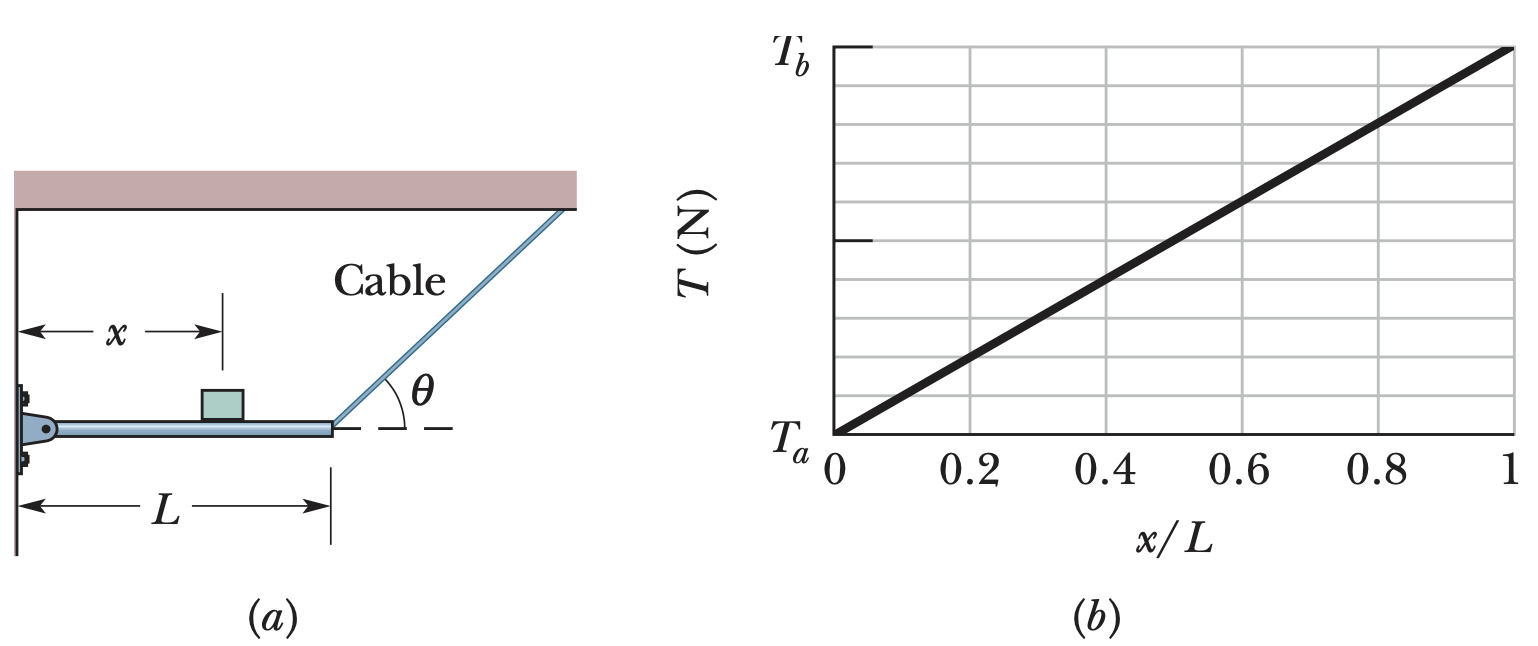
\includegraphics[scale=0.4]{Qfig15-3-20220502.png}
  \caption{문제 3}
  \label{fig:3}
\end{figure}
\begin{itemize}
\item[(가)] 각도 $\theta$
\item[(나)] 질량 $m_b$
\item[(다)] 질량 $m_p$를 각각 구하여라. 
\end{itemize}

\noindent {\bf 풀이 : } 
작용점을 고려하여 막대에게 작용하는 힘을 그려보면 다음과 같다.
\begin{figure}[htbp]
  \centering
  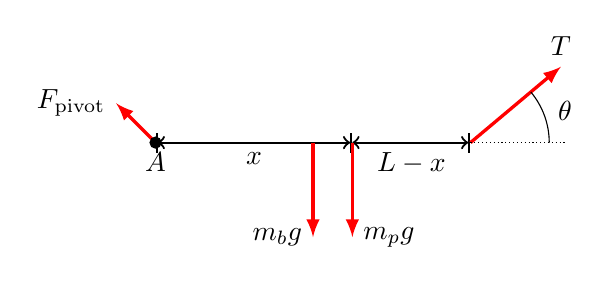
\begin{tikzpicture}
    
    \coordinate (A) at (-2,0);
    \coordinate (b) at (0,0);
    \coordinate (p) at (0.5,0);
    \coordinate (B) at (2,0);
    \draw[thick] [|<->|] (A)--(p) node [midway,below] {$x$};
    \draw[thick] [<->|] (p)--(B) node [midway,below] {$L-x$};
    \draw[red,very thick,-latex] (A)-- +(-0.5,0.5)
    node [left,black] {$F_{\mathrm{pivot}}$};
    \draw[red,very thick,-latex] (b)-- +(0,-1.2)
    node [left,black] {$m_{b}g$};
    \draw[red,very thick,-latex] (p)-- +(0,-1.2)
    node [right,black] {$m_{p}g$};
    \draw[red,very thick,-latex] (B)-- +(40:1.5)
    node [above,black] {$T$};
    \draw[densely dotted] (B)-- +(1.2,0);
    \draw[] (B)+(1,0) arc(0:40:1) (B)+(1.2,0.4)
    node[] {$\theta$};
    \draw[fill] (A) circle (2pt) node [below,black] {$A$};
  \end{tikzpicture}
  \caption{막대에 작용하는 힘}
\end{figure} 경첩에 의해 작용하는 힘 $F_{\mathrm{pivot}}$ 또한 분명 존재하지만 
이 문제에서는 중요하지 않으므로 대략적으로 그려 놓았다.
물체에 의한 중력은 $m_{p}g$, 막대에 의한 중력은 $m_{b}g$ 이고
케이블에 의한 장력을 $T$라 하자. $T$와 $x/L$에 대한
그래프를 수식적으로 표현해보면 다음과 같다.
\begin{align}\label{eq:3-1}
  \begin{split}
    T &= \left(\frac{T_b - T_a}{1-0}\right)\frac{x}{L}+T_a
    =\left(T_b - T_a\right)\frac{x}{L}+T_a.
  \end{split}
\end{align}
경첩을 회전축으로 하는 막대에 대한 돌림힘의 합은 0이다. 
이를 운동 방정식으로 표현하면
\begin{align}\label{eq:3-2}
  \sum \tau = \frac{L}{2}m_{b}g + xm_{p}g-TL\sin\theta=0
\end{align}
이다.
식~\eqref{eq:3-1}과 같이 $T$에 대해 표현하면 다음과 같다.
\begin{align}\label{eq:3-3}
  T = \frac{m_{p}g}{\sin\theta}\frac{x}{L}
  +\frac{m_{b}g}{2\sin\theta}.
\end{align}
같은 물리현상을 다루고 있으므로 식~\eqref{eq:3-1}과~\eqref{eq:3-3}은 
임의의 $x$와 $L$에 대해 성립한다. 따라서
\begin{align}
  \label{eq:3-3-1}T_b - T_a &= \frac{m_{p}g}{\sin\theta},  \\
  \label{eq:3-3-2}T_a &= \frac{m_{b}g}{2\sin\theta}
\end{align}
이다.
\begin{itemize}
  \item[(가)]
  식~\eqref{eq:3-3-1}, \eqref{eq:3-3-2}로부터
  \begin{align}
    T_b+T_a = \frac{m_{b}g+m_{p}g}{\sin\theta}
  \end{align}
  이고 $\sin\theta$는
  \begin{align}
    \sin\theta = \frac{m_{b}g+m_{p}g}{T_b+T_a}
    =\frac{(m_b+m_p)g}{T_b+T_a}
  \end{align}
  이다. 수치를 넣어 계산해보면
  \begin{align}
    \begin{split}
      \sin\theta = \frac{(61.22\,\mathrm{kg})
      (9.806\,\mathrm{m.s^2})}
      {(700\,\mathrm{N})+(500\,\mathrm{N})}
      = 0.500
    \end{split}
  \end{align}
  을 얻는다. 따라서 $\theta$는 $30.00^\circ$이다.
  \item[(나)] 
    식~\eqref{eq:3-3-2}로부터 $T_a$는 다음과 같이 표현할 수 있다.
    \begin{align}
      T_a &= \frac{m_{b}g}{2\sin\theta}
      = \frac{m_{b}(T_b+T_a)}{2(m_b+m_p)}.
    \end{align}
    따라서 $m_b$이므로
    \begin{align}
      m_b = \frac{2T_a(m_b+m_p)}{T_b+T_a}
    \end{align}
  이다. 수치를 넣어서 계산해보면 다음과 같다.
  \begin{align}
    \begin{split}
      m_b &= \frac{2(500\,\mathrm{N})(61.22\,\mathrm{kg})}
      {(700\,\mathrm{N})+(500\,\mathrm{N})} \\
      &= 51.01\,\mathrm{kg}.
    \end{split}
  \end{align}
  $m_b$는 $51.02\,\mathrm{kg}$이다.
  \item[(다)]
  $m_b+m_p=61.22$ kg이므로 $m_p$는 $10.20\,\mathrm{kg}$이다.
\end{itemize}

\vspace{1.cm}

\noindent {\bf 문제 4. (40pt)}
그림~\ref{fig:4}는 질량 103 kg인 균일한 통나무를 반지름 1.20 mm인 두
개의 강철선 $A$와 $B$로 매달아 놓은 것이다. 처음에는 길이가 2.50 m인
줄 $A$가 줄보다 2.00 mm만큼 짧았으나 지금은 통나무가 수평하게 되었다. 
$B$보다 
\begin{figure}[ht]
  \centering
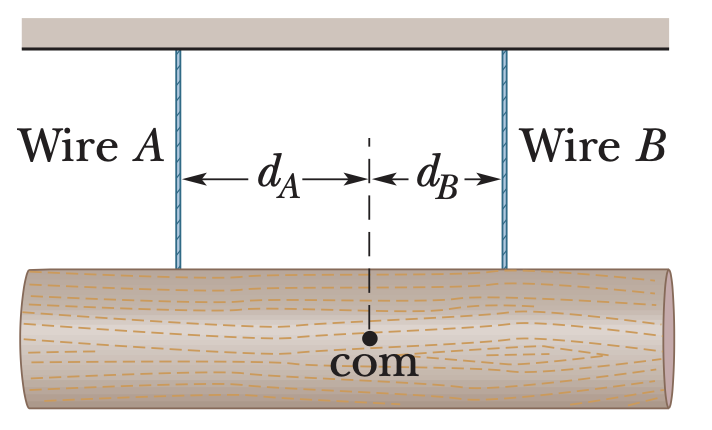
\includegraphics[scale=0.25]{Qfig15-4-20220502.png}
  \caption{문제 4}
  \label{fig:4}
\end{figure}
\begin{itemize}
\item[(가)] 줄 $A$와
\item[(나)] 줄 $B$가 통나무에 가하는 힘은 각각 얼마인가? 
\item[(다)] $d_A/d_B$의 비율은 얼마인가? 
\end{itemize}

\noindent {\bf 풀이 : } {\color{blue} (이 문제를 수치적으로 풀기
위해서는 철에 대한 영의 모듈
\begin{align}
Y = 200\times 10^9\,\mathrm{N/m^2}  
\end{align}
이 주어져야 한다.)} $Y$값을 주지 않았으므로, $Y$만 써놓아도 괜찮다.
\\
통나무에 작용하는 힘을 다음과 같이 그릴 수 있다.
\begin{figure}[htbp]
  \centering
  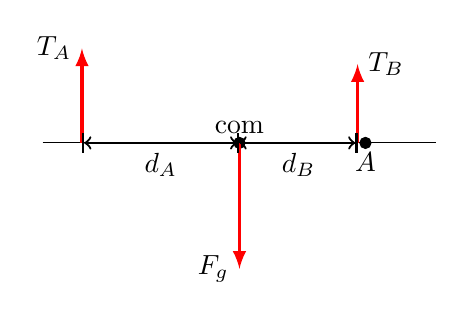
\begin{tikzpicture}
    \coordinate (O) at (0,0);
    \coordinate (A) at (-2,0);
    \coordinate (B) at (1.5,0);
    \draw (-2.5,0) -- (2.5,0);


    \draw[fill] (O) circle (2pt) node [above,black] {com};
    \draw[red,very thick,-latex] (A) -- +(0,1.2) 
    node [left,black] {$T_A$};
    \draw[red,very thick,-latex] (O)-- +(0,-1.6)
    node [left,black] {$F_g$};
    \draw[fill] (1.6,0) circle (2pt) node [below,black] {$A$};
    \draw[red,very thick,-latex] (B)-- +(0,1)
    node [right,black] {$T_B$};
    \draw[thick] [|<->|] (A)--(O) node [midway,below] {$d_A$};
    \draw[thick] [<->|] (O)--(B) node [midway,below] {$d_B$};
  \end{tikzpicture}
  \caption{통나무에 작용하는 힘}
\end{figure} 

통나무의 운동방정식은 다음과 같이 적을 수 있다.
\begin{align}
  \label{eq:4-1-1}\sum F    &= T_A + T_B - F_g   = 0 \\
  \label{eq:4-1-2}\sum \tau &= T_A d_A - T_B d_B = 0
\end{align}
\begin{itemize}
  \item[(가)] 
  강철선 $A$의 원래 길이를 $L_A$, 늘어난 길이를 $\Delta L_A$, 
  강철선 $B$의 원래 길이를 $L_B$, 늘어난 길이를 $\Delta L_B$, 
  두 강철선의 단면적을 $A$라 하자.
  라고 하자. 강철선에 걸리는 장력이 변형력이므로
  \begin{align}  \label{eq:4-2}
    \frac{T_A }{A} = Y\frac{\Delta L_A}{L_A},\,\,\,
    \frac{T_B }{A} = Y\frac{\Delta L_B}{L_B}
  \end{align}
  $r$은 강철선의 지름이고
  $Y$는 강철의 영률로 $200\times 10^9\mathrm{N/m^2}$이다.
  강철선은 처음에 길이 차이가 있었다. 그 길이 차를 $l$라 하면
  \begin{align}\label{eq:4-3}
    L_A = L_B - l
  \end{align}  
  이다. 통나무에 매달려 두 강철선의 길이가 같아졌으므로 
  \begin{align}
    \Delta L_A= \Delta L_B + l
  \end{align}
  이고 식~\eqref{eq:4-1-1}와~\eqref{eq:4-2}로부터
  \begin{align}
    \frac{ T_AL_A }{YA } = \frac{T_B L_B }{Y A} + l
  \end{align}
  을 얻는다. 식~\eqref{eq:4-3}과 함께 $T_A$에 대해 정리하면
  \begin{align}
    T_A =  \frac{F_gL_B + YAl}{L_A+L_B}
    =\frac{L_Bmg + YAl}{L_A+L_B}
  \end{align}
  이다. 여기서 $m$은 통나무의 질량이다. 
   $A$는 강철선의 단면적이므로 $A = \pi r^2$이다.
  처음 길이 차 $l$는 $L_1$, $L_2$에 비해
  무시할 수 있을 만큼 작으므로 $L_1=L_2$라 하자. 수치를 넣어 정리하면
  \begin{align}
    \begin{split}
      T_A 
      &=\frac{(2.50\,\mathrm{m})(103\,\mathrm{kg})
      (9.80\,\mathrm{m/s^2})  
      + (200\times 10^9\,\mathrm{N/m^2})
      \pi(1.20\times 10^{-3}\,\mathrm{m})^2
      (2.00\times 10^{-3}\,\mathrm{m})}
      {(2.50\,\mathrm{m})+(2.50\,\mathrm{m})} \\
      &=867\,\mathrm{N}.
    \end{split}
  \end{align}
  줄 $A$가 통나무에 가하는 힘은 $867\,\mathrm{N}$이다.
  \item[(나)]
  식~\eqref{eq:4-1-1}으로부터
  \begin{align}
    T_B = F_g - T_A
    =mg - \frac{L_Bmg + YAl}{L_A+L_B}
    =\frac{L_Amg - YAl}{L_A+L_B}
  \end{align}
  이고 수치를 넣어 대입하면,
  \begin{align}
    \begin{split}
      T_B &=
      \frac{(2.50\,\mathrm{m})(103\,\mathrm{kg})
      (9.80\,\mathrm{m/s^2})  
      - (200\times 10^9\,\mathrm{N/m^2})
      \pi(1.20\times 10^{-3}\,\mathrm{m})^2
      (2.00\times 10^{-3}\,\mathrm{m})}
      {(2.50\,\mathrm{m})+(2.50\,\mathrm{m})} \\
      &=143\,\mathrm{N}.
    \end{split}
  \end{align}
  이다. 줄 $B$가 통나무에 가하는 힘은 $143\,\mathrm{N}$이다.
  \item[(다)]
  식~\eqref{eq:4-1-2}으로부터
  \begin{align}
    \begin{split}
      \frac{d_A}{d_B} &= \frac{T_B}{T_A}
      =\frac{L_B mg-YAl}{L_Amg + YAl} \\
      &= \frac{(2.50\,\mathrm{m})(103\,\mathrm{kg})
      (9.80\,\mathrm{m/s^2})  
      - (200\times 10^9\,\mathrm{N/m^2})
      \pi(1.20\times 10^{-3}\,\mathrm{m})^2
      (2.00\times 10^{-3}\,\mathrm{m})}
      {(2.50\,\mathrm{m})(103\,\mathrm{kg})
      (9.80\,\mathrm{m/s^2})  
      + (200\times 10^9\,\mathrm{N/m^2})
      \pi(1.20\times 10^{-3}\,\mathrm{m})^2
      (2.00\times 10^{-3}\,\mathrm{m})} \\
      &= 0.165
    \end{split}
  \end{align}
  이다.
\end{itemize}

\end{document}